\documentclass[9pt]{beamer}
\mode<presentation>

% Theme choice:
\usetheme{Madrid}%Darmstadt 
\usepackage{xcolor}
\definecolor{mGreen}{rgb}{0,0.6,0}
\definecolor{mRed}{rgb}{0.6,0,0}
\usecolortheme[RGB={0,100,50}]{structure}
 \usefonttheme{structurebold} 
\setbeamercovered{invisible}
%\setbeamertemplate{navigation symbols}{}
\usepackage{dynblocks}
\usepackage{textpos}
\usepackage{amsfonts}
\usepackage{amsmath}
\usepackage{amssymb}
\usepackage{amsthm}
\usepackage{listings}
\usepackage{tikz}
\usepackage{pgfplots}
\pgfplotsset{compat=1.18}
\usetikzlibrary{
  arrows.meta,
  positioning,
  calc,
  fit,
  shapes.geometric,
  shapes.misc
}
\newtheorem{teorema}{Teorema}\usepackage{mathtools}
\renewcommand{\proofname}{Prova}
\usepackage[portuguese]{babel}

\uselanguage{Portuguese}
\languagepath{Portuguese}

\deftranslation[to=Portuguese]{Theorem}{Teorema}
\deftranslation[to=Portuguese]{Lemma}{Lema}
\deftranslation[to=Portuguese]{Corollary}{Corolário}
\deftranslation[to=Portuguese]{Proof}{Prova}

\usepackage{dutchcal}
\usepackage[utf8]{inputenc}
\usepackage[T1]{fontenc}
\usepackage{booktabs}
\usepackage[affil-it]{authblk} 
\usepackage{etoolbox}
\usepackage{lmodern}
\usepackage[pscoord]{eso-pic}
\usepackage{hyperref}

\makeatletter
\patchcmd{\@maketitle}{\LARGE \@title}{\fontsize{18}{19.2}\selectfont\@title}{}{}
\makeatother

\renewcommand\Authfont{\fontsize{12}{14.4}\selectfont}
\renewcommand\Affilfont{\fontsize{9}{10.8}\itshape}

% Estilos TikZ reutilizáveis (tema verde da apresentação)
\tikzset{
  softbox/.style={
    draw=structure.fg,
    fill=structure.fg!12,
    rounded corners=3pt,
    align=center,
    font=\small,
    minimum height=0.9cm,
    inner sep=4pt
  },
  softboxalert/.style={
    draw=mRed,
    fill=mRed!10,
    rounded corners=3pt,
    align=center,
    font=\small,
    minimum height=0.9cm,
    inner sep=4pt
  },
  softcore/.style={
    draw=structure.fg,
    fill=structure.fg!25,
    circle,
    align=center,
    font=\bfseries\small,
    minimum size=1.55cm,
    inner sep=2pt
  },
  softarrow/.style={
    -{Latex[length=2.2mm]},
    thick,
    structure.fg
  },
  softarrowalert/.style={
    -{Latex[length=2.2mm]},
    thick,
    mRed
  },
  softlabel/.style={font=\scriptsize\bfseries, text=structure.fg},
  % Mockups de interface gráfica
  guiwin/.style={
    draw=#1!70!black,
    fill=white,
    rounded corners=2pt,
    inner sep=0pt,
    thick
  },
  guibar/.style={
    draw=none,
    fill=#1,
    minimum height=0.32cm,
    inner sep=1pt,
    font=\tiny\bfseries,
    text=white,
    anchor=north west
  },
  guibtn/.style={
    circle,
    fill=#1,
    minimum size=0.14cm,
    inner sep=0pt
  },
  guiphone/.style={
    draw=#1!80!black,
    fill=black!85,
    rounded corners=6pt, 
    thick,
    inner sep=2pt
  },
  qcard/.style={
    draw=structure.fg!70!black,
    fill=structure.fg!5,
    rounded corners=4pt,
    thick,
    text width=4.8cm,
    minimum height=1.5cm,
    align=left,
    inner sep=6pt
  }
}

% Title page details: 
\title[Presentation]{Da Compreensão Conceitual dos Fluxos de Processo (Linear, Iterativo, Evolucionário e Paralelo) à Aplicação Prática dos Modelos Prescritivos (Cascata, Prototipação e Espiral)} %add title

\institute[UniRV]{\large PROCESSO DE SOFTWARE --- Professor: Me. Sergio Souza Novak --- Faculdade de Engenharia de Software}
% \titlegraphic{\includegraphics[width=5cm]{msu.eps}}
\titlegraphic{
\includegraphics[width=5cm]{Universidade_de_Rio_Verde.jpg}}
\date{}
 
% Logo only on title page
%\logo{
\includegraphics[width=1cm,keepaspectratio]{Logo.png}}


\begin{document}

% Title page frame
\frame[plain]{\titlepage}
%logo
\AddToShipoutPictureFG{
    \put(\LenToUnit{.92\paperwidth},
    \LenToUnit{.185\paperheight})
    {\vtop{{\null}
    \makebox{
\includegraphics[width=.8cm,keepaspectratio]{Universidade_de_Rio_Verde.jpg}}}}}

\begin{frame}{Sumário}
  \tableofcontents
\end{frame}

\section{O Processo de Software}
\begin{frame}[fragile]{Hierarquia do Processo de Software}
  \vspace{0.3cm}
  \centering
  \begin{tikzpicture}[scale=0.85, every node/.style={transform shape}]
    % Camada 1: Processo (base estreita)
    \filldraw[fill=blue!10, draw=blue!80!black, thick] (-0.5,0) -- (0.5,0) -- (1.3,1.2) -- (-1.3,1.2) -- cycle;
    \node[font=\bfseries\footnotesize, blue!80!black] at (0, 0.6) {Processo};

    % Camada 2: Atividades
    \filldraw[fill=blue!20, draw=blue!80!black, thick] (-1.3,1.2) -- (1.3,1.2) -- (2.15,2.6) -- (-2.15,2.6) -- cycle;
    \node[font=\bfseries\small, blue!80!black] at (0, 1.9) {Atividades Metodológicas};

    % Camada 3: Ações
    \filldraw[fill=blue!30, draw=blue!80!black, thick] (-2.15,2.6) -- (2.15,2.6) -- (3.05,4.0) -- (-3.05,4.0) -- cycle;
    \node[font=\bfseries\large, blue!80!black] at (0, 3.3) {Ações de Engenharia};

    % Camada 4: Tarefas (topo largo)
    \filldraw[fill=blue!40, draw=blue!80!black, thick] (-3.05,4.0) -- (3.05,4.0) -- (4,5.5) -- (-4,5.5) -- cycle;
    \node[font=\bfseries\Large, blue!80!black] at (0, 4.75) {Tarefas};
  \end{tikzpicture}
  
  \vspace{0.4cm}
  \small
  \begin{itemize}
    \item \textbf{Processo}: Define a estrutura global.
    \item \textbf{Atividades}: Fases metodológicas amplas (ex: Comunicação, Modelagem).
    \item \textbf{Ações}: Passos dentro de uma atividade (ex: Projeto arquitetural).
    \item \textbf{Tarefas}: Trabalho diário específico da equipe (ex: Criar diagrama).
  \end{itemize}
\end{frame}

\begin{frame}[fragile]{Exemplo Prático da Hierarquia}
  \vspace{0.3cm}
  \centering
  \begin{tikzpicture}[every node/.style={transform shape}, rounded corners=2pt, thick]
    % Processo
    \node[draw=blue!80!black, fill=blue!10, text width=9.5cm, inner sep=6pt, align=left] (proc) at (0,4.5) {
        \textbf{\textcolor{blue!80!black}{1. Processo de Software}}\\
        Exemplo: \textit{Desenvolvimento com Processo Ágil (ex: Scrum)}
    };

    % Atividade
    \node[draw=blue!80!black, fill=blue!20, text width=8.5cm, inner sep=6pt, align=left] (ativ) at (0.5,3.0) {
        \textbf{\textcolor{blue!80!black}{2. Atividade Metodológica}}\\
        Exemplo: \textit{Comunicação (Levantamento de Requisitos)}
    };
    \draw[->, thick, blue!80!black] ([xshift=0.5cm, yshift=-0.1cm]proc.south west) |- (ativ.west);

    % Ação
    \node[draw=blue!80!black, fill=blue!30, text width=7.5cm, inner sep=6pt, align=left] (acao) at (1.0,1.5) {
        \textbf{\textcolor{blue!80!black}{3. Ação de Engenharia}}\\
        Exemplo: \textit{Elicitação e Análise de Requisitos}
    };
    \draw[->, thick, blue!80!black] ([xshift=0.5cm, yshift=-0.1cm]ativ.south west) |- (acao.west);

    % Tarefas
    \node[draw=blue!80!black, fill=blue!40, text width=6.5cm, inner sep=6pt, align=left] (tar) at (1.5,-0.3) {
        \textbf{\textcolor{black}{4. Tarefas (O Trabalho Diário)}}\\
        \vspace{0.1cm}
        {\footnotesize
        \textbullet\ Agendar reunião com o diretor.\\
        \textbullet\ Conduzir entrevista sobre necessidades.\\
        \textbullet\ Escrever as \textit{User Stories}.\\
        \textbullet\ Validar as anotações com a equipe.}
    };
    \draw[->, thick, blue!80!black] ([xshift=0.5cm, yshift=-0.1cm]acao.south west) |- (tar.west);
  \end{tikzpicture}
\end{frame}


\begin{frame}{Atividades de apoio de um processo}
  \vspace{0.4cm}
  \centering
  \begin{tikzpicture}[node distance=0.38cm, scale=1, every node/.style={transform shape}]
    \node [softbox] (com) {Comunicação};
    \node [softbox, right=of com] (plan) {Planejamento};
    \node [softbox, right=of plan] (mod) {Modelagem};
    \node [softbox, right=of mod] (const) {Construção};
    \node [softbox, right=of const] (entr) {Entrega};
    
    \draw [softarrow] (com) -- (plan);
    \draw [softarrow] (plan) -- (mod);
    \draw [softarrow] (mod) -- (const);
    \draw [softarrow] (const) -- (entr);
    
    % Entrada e saída indicativas
    \draw [softarrow] ($(com.west)+(-0.4,0)$) -- (com.west);
    \draw [softarrow] (entr.east) -- ($(entr.east)+(0.4,0)$);
  \end{tikzpicture}
  \vspace{0.4cm}

\end{frame}


\begin{frame}{Processo de software}
 \begin{center}
  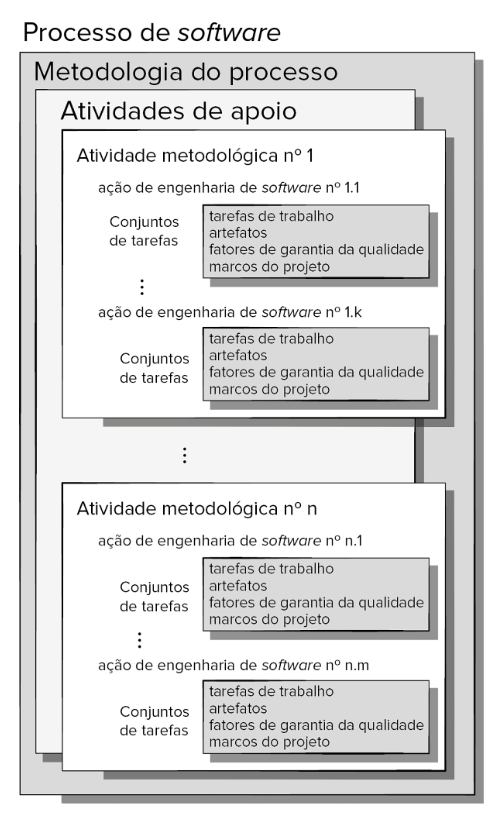
\includegraphics[width=0.4\textwidth]{./images/img1.png}
\end{center}
\end{frame}
\section{Fluxos de Processo}

\subsection{Fluxo Linear}
\begin{frame}{Estrutura do Processo de Software}
  \begin{columns}
    \begin{column}{0.55\textwidth}
      \small
      O processo de software é uma estrutura que organiza as atividades de desenvolvimento:
      \vspace{0.2cm}
      \begin{itemize}
        \item \textbf{Atividade Metodológica}: Ações de trabalho que determinam o relacionamento entre si e com o processo global.
        \item \textbf{Ações de Engenharia}: Conjuntos de tarefas focadas em objetivos específicos do projeto.
        \item \textbf{Conjunto de Tarefas}: Define o trabalho real:
          \begin{itemize}
            \item Tarefas de trabalho a serem completadas.
            \item Artefatos de software produzidos.
            \item Fatores de garantia da qualidade exigidos.
            \item Marcos (milestones) para indicar progresso.
          \end{itemize}
      \end{itemize}
    \end{column}
    \begin{column}{0.45\textwidth}
      \centering
      \begin{tikzpicture}[node distance=0.7cm, scale=0.8, every node/.style={transform shape}]
        \node [softcore] (proc) {Processo};
        \node [softbox, below=of proc] (ativ) {Atividade\\Metodológica};
        \node [softbox, below=of ativ] (acao) {Ação de\\Engenharia};
        \node [softbox, below=of acao] (tarefa) {Conjunto de\\Tarefas};
        
        \draw [softarrow] (proc) -- (ativ);
        \draw [softarrow] (ativ) -- (acao);
        \draw [softarrow] (acao) -- (tarefa);
      \end{tikzpicture}
    \end{column}
  \end{columns}
\end{frame}

\begin{frame}{Fluxo de Processo Linear}
  Um \textbf{fluxo de processo linear} executa cada uma das cinco atividades metodológicas em sequência direta, iniciando na comunicação e concluindo na entrega.

  \vspace{0.4cm}
  \centering
  \begin{tikzpicture}[node distance=0.18cm, scale=0.78, every node/.style={transform shape}]
    \node [softbox] (com) {Comunicação};
    \node [softbox, right=of com] (plan) {Planejamento};
    \node [softbox, right=of plan] (mod) {Modelagem};
    \node [softbox, right=of mod] (const) {Construção};
    \node [softbox, right=of const] (entr) {Entrega};
    
    \draw [softarrow] (com) -- (plan);
    \draw [softarrow] (plan) -- (mod);
    \draw [softarrow] (mod) -- (const);
    \draw [softarrow] (const) -- (entr);
    
    % Entrada e saída indicativas
    \draw [softarrow] ($(com.west)+(-0.4,0)$) -- (com.west);
    \draw [softarrow] (entr.east) -- ($(entr.east)+(0.4,0)$);
  \end{tikzpicture}
  \vspace{0.4cm}

  \begin{itemize}
    \item \textbf{Sequência Rígida}: Nenhuma etapa é iniciada até que a anterior esteja concluída.
    \item \textbf{Adequabilidade}: Ideal para projetos simples, bem compreendidos e com requisitos altamente estáveis que não sofrerão alterações durante o desenvolvimento.
  \end{itemize}
\end{frame}

\begin{frame}{Exemplo Prático de Fluxo Linear}

\small

\textbf{Cenário:} Desenvolvimento de um
\textit{Site Institucional Estático} para uma clínica médica.

\vspace{0.35cm}

\begin{tikzpicture}[
    >=stealth,
    node distance=0.35cm,
    etapa/.style={
        draw=blue!60!black,
        fill=blue!8,
        rounded corners=2pt,
        minimum width=2.25cm,
        minimum height=0.75cm,
        align=center,
        font=\scriptsize\bfseries
    },
    exemplo/.style={
        draw=gray!60,
        fill=gray!8,
        rounded corners=2pt,
        text width=2.25cm,
        minimum height=1.35cm,
        align=left,
        font=\fontsize{5.8}{7}\selectfont,
        inner sep=5pt
    },
    seta/.style={
        ->,
        very thick,
        blue!60!black
    }
]

% ============================================================
% ETAPAS
% ============================================================

\node[etapa] (com) {1. Comunicação};
\node[etapa, right=of com] (plan) {2. Planejamento};
\node[etapa, right=of plan] (model) {3. Modelagem\\(Design)};
\node[etapa, right=of model] (const) {4. Construção};
\node[etapa, right=of const] (ent) {5. Entrega};

% ============================================================
% SETAS
% ============================================================

\draw[seta] (com) -- (plan);
\draw[seta] (plan) -- (model);
\draw[seta] (model) -- (const);
\draw[seta] (const) -- (ent);

% ============================================================
% EXEMPLOS
% ============================================================

\node[exemplo, below=0.25cm of com] (ecom) {
    \textbf{Ação: Elicitação}\\
    \textbf{Tarefas:}\\
    • Identificar serviços\\
    • Coletar fotos da clínica\\
    • Definir cores e estilo
};

\node[exemplo, below=0.25cm of plan] (eplan) {
    \textbf{Ação: Estimativa}\\
    \textbf{Tarefas:}\\
    • Definir prazo (1 semana)\\
    • Orçar custos\\
    • Escolher hospedagem
};

\node[exemplo, below=0.25cm of model] (emodel) {
    \textbf{Ação: Design UI}\\
    \textbf{Tarefas:}\\
    • Criar wireframe inicial\\
    • Elaborar visual da página\\
    • Obter aprovação
};

\node[exemplo, below=0.25cm of const] (econst) {
    \textbf{Ação: Codificação}\\
    \textbf{Tarefas:}\\
    • Codificar HTML/CSS\\
    • Organizar estrutura\\
    • Otimizar imagens
};

\node[exemplo, below=0.25cm of ent] (eent) {
    \textbf{Ação: Implantação}\\
    \textbf{Tarefas:}\\
    • Publicar na hospedagem\\
    • Testar links e formulário\\
    • Homologar com cliente
};

% ============================================================
% FLUXO INFERIOR
% ============================================================

\draw[
    ->,
    very thick,
    green!50!black
]
(ecom.south) -- ++(0,-0.35)
-| (eplan.south);

\end{tikzpicture}

\vspace{0.25cm}

\begin{center}
\colorbox{blue!10}{
    \parbox{0.9\textwidth}{
        \centering
        \scriptsize
        \textbf{Fluxo linear:}
        Comunicação $\rightarrow$
        Planejamento $\rightarrow$
        Modelagem $\rightarrow$
        Construção $\rightarrow$
        Entrega
    }
}
\end{center}
\end{frame}

\begin{frame}{Estrutura da Atividade Metodológica: Construção}
  \small
  Exemplo de instanciação da hierarquia do processo para a atividade de \textbf{Construção}:

  \vspace{0.1cm}
  \centering
  \begin{tikzpicture}[
      >=stealth,
      scale=0.82,
      every node/.style={transform shape},
      apoio/.style={draw=gray!30, fill=gray!5, rounded corners=3pt, thick},
      moldura/.style={draw=blue!50!black, fill=blue!3, rounded corners=3pt, thick},
      acao/.style={draw=blue!70!black, fill=white, rounded corners=3pt, thick, text width=6.2cm, inner sep=6pt},
      conjunto/.style={draw=gray!50, fill=gray!8, rounded corners=2pt, text width=5.8cm, font=\fontsize{6.5}{7.5}\selectfont, inner sep=4pt}
  ]
      % Atividades de Apoio (Fundo overlapping)
      \node[apoio, minimum width=7.2cm, minimum height=6.2cm] (apoio2) at (0.12, -0.12) {};
      \node[apoio, minimum width=7.2cm, minimum height=6.2cm, label={[shift={(0.2,-0.45)}]north west:\scriptsize\textbf{Atividades de Apoio (Gerenciamento, Qualidade)}}] (apoio1) at (0, 0) {};

      % Atividade Metodológica (Frente)
      \node[moldura, minimum width=7.0cm, minimum height=5.6cm, below=0.35cm of apoio1.north, anchor=north] (ativ) {};
      \node[anchor=north west, font=\scriptsize\bfseries, text=blue!80!black] at (ativ.north west) {Atividade Metodológica: Construção};

      % Ação 1: Codificação
      \node[acao, below=0.45cm of ativ.north, anchor=north] (acao1) {
          \scriptsize \textbf{Ação de Eng. de Software: Codificação}\\[1mm]
          \begin{tikzpicture}[every node/.style={transform shape}]
              \node[conjunto] {
                  \textbf{Conjunto de Tarefas (Codificação):}\\
                  • \textbf{Tarefas de trabalho:} Codificar a estrutura (HTML) e estilo (CSS)\\
                  • \textbf{Artefatos produzidos:} Arquivos \texttt{.html}, \texttt{.css} e scripts\\
                  • \textbf{Garantia da qualidade:} Validação de padrões W3C e linting\\
                  • \textbf{Marcos de progresso:} Protótipo visual responsivo concluído
              };
          \end{tikzpicture}
      };

      % Ação 2: Testes
      \node[acao, below=0.3cm of acao1.south, anchor=north] (acao2) {
          \scriptsize \textbf{Ação de Eng. de Software: Testes}\\[1mm]
          \begin{tikzpicture}[every node/.style={transform shape}]
              \node[conjunto] {
                  \textbf{Conjunto de Tarefas (Testes):}\\
                  • \textbf{Tarefas de trabalho:} Executar testes de navegabilidade e links\\
                  • \textbf{Artefatos produzidos:} Relatório de testes e registro de erros\\
                  • \textbf{Garantia da qualidade:} Cobertura de testes em múltiplos navegadores\\
                  • \textbf{Marcos de progresso:} Código homologado e pronto para entrega
              };
          \end{tikzpicture}
      };
  \end{tikzpicture}
\end{frame}

\begin{frame}{Estrutura da Atividade Metodológica: Comunicação}
  \small
  Exemplo de instanciação da hierarquia do processo para a atividade de \textbf{Comunicação}:

  \vspace{0.1cm}
  \centering
  \begin{tikzpicture}[
      >=stealth,
      scale=0.82,
      every node/.style={transform shape},
      apoio/.style={draw=gray!30, fill=gray!5, rounded corners=3pt, thick},
      moldura/.style={draw=blue!50!black, fill=blue!3, rounded corners=3pt, thick},
      acao/.style={draw=blue!70!black, fill=white, rounded corners=3pt, thick, text width=6.2cm, inner sep=6pt},
      conjunto/.style={draw=gray!50, fill=gray!8, rounded corners=2pt, text width=5.8cm, font=\fontsize{6.5}{7.5}\selectfont, inner sep=4pt}
  ]
      % Atividades de Apoio (Fundo overlapping)
      \node[apoio, minimum width=7.2cm, minimum height=6.2cm] (apoio2) at (0.12, -0.12) {};
      \node[apoio, minimum width=7.2cm, minimum height=6.2cm, label={[shift={(0.2,-0.45)}]north west:\scriptsize\textbf{Atividades de Apoio (Gerenciamento, Qualidade)}}] (apoio1) at (0, 0) {};

      % Atividade Metodológica (Frente)
      \node[moldura, minimum width=7.0cm, minimum height=5.6cm, below=0.35cm of apoio1.north, anchor=north] (ativ) {};
      \node[anchor=north west, font=\scriptsize\bfseries, text=blue!80!black] at (ativ.north west) {Atividade Metodológica: Comunicação};

      % Ação 1: Concepção
      \node[acao, below=0.45cm of ativ.north, anchor=north] (acao1) {
          \scriptsize \textbf{Ação de Eng. de Software: Concepção (Elicitação)}\\[1mm]
          \begin{tikzpicture}[every node/.style={transform shape}]
              \node[conjunto] {
                  \textbf{Conjunto de Tarefas (Concepção):}\\
                  • \textbf{Tarefas de trabalho:} Realizar reuniões e coletar requisitos iniciais\\
                  • \textbf{Artefatos produzidos:} Atas de reunião, lista preliminar de requisitos\\
                  • \textbf{Garantia da qualidade:} Validação de escopo com os principais stakeholders\\
                  • \textbf{Marcos de progresso:} Necessidades e escopo inicial documentados
              };
          \end{tikzpicture}
      };

      % Ação 2: Negociação
      \node[acao, below=0.3cm of acao1.south, anchor=north] (acao2) {
          \scriptsize \textbf{Ação de Eng. de Software: Negociação de Escopo}\\[1mm]
          \begin{tikzpicture}[every node/.style={transform shape}]
              \node[conjunto] {
                  \textbf{Conjunto de Tarefas (Negociação):}\\
                  • \textbf{Tarefas de trabalho:} Alinhar expectativas, prazos e custos do projeto\\
                  • \textbf{Artefatos produzidos:} Proposta técnica, termo de especificações acordadas\\
                  • \textbf{Garantia da qualidade:} Análise de viabilidade técnica e financeira\\
                  • \textbf{Marcos de progresso:} Contrato assinado ou escopo final formalizado
              };
          \end{tikzpicture}
      };
  \end{tikzpicture}
\end{frame}

\begin{frame}{Estrutura da Atividade Metodológica: Entrega}
  \small
  Exemplo de instanciação da hierarquia do processo para a atividade de \textbf{Entrega} (Implantação):

  \vspace{0.1cm}
  \centering
  \begin{tikzpicture}[
      >=stealth,
      scale=0.82,
      every node/.style={transform shape},
      apoio/.style={draw=gray!30, fill=gray!5, rounded corners=3pt, thick},
      moldura/.style={draw=blue!50!black, fill=blue!3, rounded corners=3pt, thick},
      acao/.style={draw=blue!70!black, fill=white, rounded corners=3pt, thick, text width=6.2cm, inner sep=6pt},
      conjunto/.style={draw=gray!50, fill=gray!8, rounded corners=2pt, text width=5.8cm, font=\fontsize{6.5}{7.5}\selectfont, inner sep=4pt}
  ]
      % Atividades de Apoio (Fundo overlapping)
      \node[apoio, minimum width=7.2cm, minimum height=6.2cm] (apoio2) at (0.12, -0.12) {};
      \node[apoio, minimum width=7.2cm, minimum height=6.2cm, label={[shift={(0.2,-0.45)}]north west:\scriptsize\textbf{Atividades de Apoio (Gerenciamento, Qualidade)}}] (apoio1) at (0, 0) {};

      % Atividade Metodológica (Frente)
      \node[moldura, minimum width=7.0cm, minimum height=5.6cm, below=0.35cm of apoio1.north, anchor=north] (ativ) {};
      \node[anchor=north west, font=\scriptsize\bfseries, text=blue!80!black] at (ativ.north west) {Atividade Metodológica: Entrega};

      % Ação 1: Implantação
      \node[acao, below=0.45cm of ativ.north, anchor=north] (acao1) {
          \scriptsize \textbf{Ação de Eng. de Software: Implantação (Deployment)}\\[1mm]
          \begin{tikzpicture}[every node/.style={transform shape}]
              \node[conjunto] {
                  \textbf{Conjunto de Tarefas (Implantação):}\\
                  • \textbf{Tarefas de trabalho:} Publicar arquivos no servidor e configurar DNS\\
                  • \textbf{Artefatos produzidos:} Site no ar em ambiente de produção\\
                  • \textbf{Garantia da qualidade:} Testes de fumaça pós-deploy e validação de SSL\\
                  • \textbf{Marcos de progresso:} Site público e acessível de forma estável
              };
          \end{tikzpicture}
      };

      % Ação 2: Feedback
      \node[acao, below=0.3cm of acao1.south, anchor=north] (acao2) {
          \scriptsize \textbf{Ação de Eng. de Software: Feedback e Suporte}\\[1mm]
          \begin{tikzpicture}[every node/.style={transform shape}]
              \node[conjunto] {
                  \textbf{Conjunto de Tarefas (Feedback):}\\
                  • \textbf{Tarefas de trabalho:} Apresentar ao cliente e coletar avaliações/ajustes\\
                  • \textbf{Artefatos produzidos:} Termo de recebimento, lista de melhorias futuras\\
                  • \textbf{Garantia da qualidade:} Avaliação da satisfação e checklist de aceitação\\
                  • \textbf{Marcos de progresso:} Homologação final e encerramento do projeto
              };
          \end{tikzpicture}
      };
  \end{tikzpicture}
\end{frame}

\subsection{Fluxo Iterativo}
\begin{frame}{Fluxo de Processo Iterativo}
  Um \textbf{fluxo de processo iterativo} repete uma ou mais atividades metodológicas (sendo executadas em ciclos) antes de prosseguir para a próxima, permitindo o refinamento contínuo do software.

  \vspace{0.4cm}
  \centering
  \begin{tikzpicture}[
      node distance=0.18cm, 
      scale=0.78, 
      every node/.style={transform shape},
      etapa/.style={draw=blue!60!black, fill=blue!8, rounded corners=2pt, minimum width=2.1cm, minimum height=0.7cm, align=center, font=\scriptsize\bfseries},
      seta/.style={->, >=stealth, thick, blue!60!black},
      setaretorno/.style={->, >=stealth, thick, red!70!black}
  ]
    \node [etapa] (com) {Comunicação};
    \node [etapa, right=of com] (plan) {Planejamento};
    \node [etapa, right=of plan] (mod) {Modelagem};
    \node [etapa, right=of mod] (const) {Construção};
    \node [etapa, right=of const] (entr) {Entrega};
    
    \draw [seta] (com) -- (plan);
    \draw [seta] (plan) -- (mod);
    \draw [seta] (mod) -- (const);
    \draw [seta] (const) -- (entr);
    
    % Entrada e saída indicativas
    \draw [seta] ($(com.west)+(-0.4,0)$) -- (com.west);
    \draw [seta] (entr.east) -- ($(entr.east)+(0.4,0)$);

    % Retornos (Loops)
    \draw [setaretorno] (plan.south) .. controls +(0,-0.4) and +(0,-0.4) .. (com.south);
    \draw [setaretorno] (mod.south) .. controls +(0.2,-0.4) and +(-0.2,-0.4) .. (mod.south);
    \draw [setaretorno] (const.south) .. controls +(0,-0.8) and +(0,-0.8) .. (com.south);
  \end{tikzpicture}
  \vspace{0.4cm}

  \begin{itemize}
    \item \textbf{Caminhos de Retorno}: As setas vermelhas indicam loops de feedback onde o fluxo retorna a etapas anteriores para correções ou novos detalhes.
    \item \textbf{Adequabilidade}: Ideal para projetos complexos onde os requisitos não são totalmente claros no início.
  \end{itemize}
\end{frame}

\begin{frame}{Exemplo Prático de Fluxo Iterativo}
  \small
  \textbf{Cenário:} Desenvolvimento de um \textit{Aplicativo de Entrega de Comida} (Delivery).
  
  \vspace{0.2cm}
  \centering
  \begin{tikzpicture}[
      >=stealth,
      node distance=0.35cm,
      scale=0.88,
      every node/.style={transform shape},
      etapa/.style={draw=blue!60!black, fill=blue!8, rounded corners=2pt, minimum width=2.2cm, minimum height=0.7cm, align=center, font=\scriptsize\bfseries},
      exemplo/.style={draw=gray!60, fill=gray!8, rounded corners=2pt, text width=2.2cm, minimum height=1.35cm, align=left, font=\fontsize{5.8}{7}\selectfont, inner sep=4pt},
      seta/.style={->, very thick, blue!60!black},
      seta_ret/.style={->, thick, red!70!black}
  ]
      % Etapas
      \node[etapa] (com) {1. Comunicação};
      \node[etapa, right=of com] (plan) {2. Planejamento};
      \node[etapa, right=of plan] (model) {3. Modelagem};
      \node[etapa, right=of model] (const) {4. Construção};
      \node[etapa, right=of const] (ent) {5. Entrega};

      \draw[seta] (com) -- (plan);
      \draw[seta] (plan) -- (model);
      \draw[seta] (model) -- (const);
      \draw[seta] (const) -- (ent);

      % Descrições
      \node[exemplo, below=0.2cm of com] (ecom) {
          \textbf{Ação: Elicitação}\\
          \textbf{Tarefas:}\\
          • Coletar requisitos\\
          • Definir fluxos básicos\\
          • Mapear usuários
      };

      \node[exemplo, below=0.2cm of plan] (eplan) {
          \textbf{Ação: Sprints}\\
          \textbf{Tarefas:}\\
          • Criar Product Backlog\\
          • Estimar as Sprints\\
          • Atribuir tarefas
      };

      \node[exemplo, below=0.2cm of model] (emodel) {
          \textbf{Ação: Prototipagem}\\
          \textbf{Tarefas:}\\
          • Criar protótipos de tela\\
          • Modelar Banco de Dados\\
          • Testar usabilidade
      };

      \node[exemplo, below=0.2cm of const] (econst) {
          \textbf{Ação: Engenharia}\\
          \textbf{Tarefas:}\\
          • Codificar Front/Back\\
          • Integrar as APIs\\
          • Executar testes unitários
      };

      \node[exemplo, below=0.2cm of ent] (eent) {
          \textbf{Ação: Transição}\\
          \textbf{Tarefas:}\\
          • Publicar nas lojas\\
          • Monitorar em produção\\
          • Coletar avaliações
      };

      % Retornos do fluxo iterativo no cenário real
      \draw[seta_ret] (eplan.south) -- ++(0,-0.3) -| node[pos=0.25, below, font=\fontsize{5}{6}\selectfont] {1. Requisitos faltantes} (ecom.south);
      \draw[seta_ret] (emodel.south) to[out=270,in=270,looseness=2.5] node[below, font=\fontsize{5}{6}\selectfont] {2. Refinar protótipo} (emodel.south);
      \draw[seta_ret] (econst.south) -- ++(0,-0.6) -| node[pos=0.25, below, font=\fontsize{5}{6}\selectfont] {3. Erro de fluxo ou regra} (ecom.south);

  \end{tikzpicture}
\end{frame}

\subsection{Fluxo Evolucionário}
\begin{frame}[fragile]{Fluxo de Processo Evolucionário}
  O \textbf{fluxo de processo evolucionário} é circular. Ele é caracterizado pela entrega de versões cada vez mais completas do software (incrementos) a cada ciclo completo executado.

  \vspace{0.2cm}
  \centering
  \begin{tikzpicture}[
      >=stealth,
      scale=0.72,
      every node/.style={transform shape},
      etapa/.style={draw=blue!60!black, fill=blue!8, rounded corners=2pt, minimum width=2.1cm, minimum height=0.7cm, align=center, font=\scriptsize\bfseries},
      seta/.style={->, thick, blue!60!black}
  ]
      % Posicionamento Circular
      \node[etapa] (com) at ({180:2.4cm}) {Comunicação};
      \node[etapa] (plan) at ({120:2.4cm}) {Planejamento};
      \node[etapa] (mod) at ({40:2.4cm}) {Modelagem};
      \node[etapa] (const) at ({320:2.4cm}) {Construção};
      \node[etapa] (entr) at ({240:2.4cm}) {Entrega};

      % Transições circulares
      \draw[seta] (com) to[bend left=20] (plan);
      \draw[seta] (plan) to[bend left=20] (mod);
      \draw[seta] (mod) to[bend left=30] (const);
      \draw[seta] (const) to[bend left=20] (entr);
      \draw[seta] (entr) to[bend left=20] (com);

      % Fluxos externos (Entrada e liberação de incremento)
      \draw[seta] ($(com.west)+(-0.5,0)$) -- (com.west);
      \draw[seta] (entr.west) -- ($(entr.west)+(-0.7,-0.2)$) node[left, font=\scriptsize\bfseries, text=green!50!black, align=right] {Incremento\\liberado};
  \end{tikzpicture}
  \vspace{0.2cm}

  \begin{itemize}
    \item \textbf{Ciclo de Feedback Contínuo}: O software \textit{evolui} à medida que o cliente utiliza cada incremento e sugere melhorias para a próxima iteração.
    \item \textbf{Adequabilidade}: Projetos de grande porte, sistemas SaaS, startups e produtos em constante mutação.
  \end{itemize}
\end{frame}

\begin{frame}{Exemplo Prático de Fluxo Evolucionário}
  \small
  \textbf{Cenário:} Desenvolvimento de um \textit{Sistema de Gestão Escolar} (SaaS).
  
  \vspace{0.2cm}
  \centering
  \begin{tikzpicture}[
      >=stealth,
      node distance=0.35cm,
      scale=0.88,
      every node/.style={transform shape},
      etapa/.style={draw=blue!60!black, fill=blue!8, rounded corners=2pt, minimum width=2.2cm, minimum height=0.7cm, align=center, font=\scriptsize\bfseries},
      exemplo/.style={draw=gray!60, fill=gray!8, rounded corners=2pt, text width=2.2cm, minimum height=1.35cm, align=left, font=\fontsize{5.8}{7}\selectfont, inner sep=4pt},
      seta/.style={->, very thick, blue!60!black},
      seta_ret/.style={->, thick, green!50!black}
  ]
      % Etapas
      \node[etapa] (com) {1. Comunicação};
      \node[etapa, right=of com] (plan) {2. Planejamento};
      \node[etapa, right=of plan] (model) {3. Modelagem};
      \node[etapa, right=of model] (const) {4. Construção};
      \node[etapa, right=of const] (ent) {5. Entrega};

      \draw[seta] (com) -- (plan);
      \draw[seta] (plan) -- (model);
      \draw[seta] (model) -- (const);
      \draw[seta] (const) -- (ent);

      % Descrições
      \node[exemplo, below=0.2cm of com] (ecom) {
          \textbf{Ação: Requisitos do Ciclo}\\
          \textbf{Tarefas:}\\
          • Definir escopo do ciclo atual (ex: Módulo de Matrículas)\\
          • Entender regras de negócio
      };

      \node[exemplo, below=0.2cm of plan] (eplan) {
          \textbf{Ação: Plano de Entrega}\\
          \textbf{Tarefas:}\\
          • Estimar esforço do módulo\\
          • Criar cronograma do ciclo\\
          • Alocar desenvolvedores
      };

      \node[exemplo, below=0.2cm of model] (emodel) {
          \textbf{Ação: Modelagem de Telas}\\
          \textbf{Tarefas:}\\
          • Desenhar telas de matrícula\\
          • Modelar tabelas de alunos\\
          • Validar fluxo com escola
      };

      \node[exemplo, below=0.2cm of const] (econst) {
          \textbf{Ação: Desenvolvimento}\\
          \textbf{Tarefas:}\\
          • Codificar módulo de matrícula\\
          • Integrar banco de dados\\
          • Realizar testes funcionais
      };

      \node[exemplo, below=0.2cm of ent] (eent) {
          \textbf{Ação: Liberação}\\
          \textbf{Tarefas:}\\
          • Publicar o módulo em produção\\
          • Treinar equipe da secretaria\\
          • \textbf{Incremento Liberado!}
      };

      % Retorno para o próximo ciclo evolucionário (Módulo de Notas, Boletim, etc)
      \draw[seta_ret] (eent.south) -- ++(0,-0.4) -| node[pos=0.25, below, font=\fontsize{5}{6}\selectfont] {Próxima Evolução (Ex: Módulo Financeiro)} (ecom.south);

  \end{tikzpicture}
\end{frame}

\subsection{Fluxo Paralelo}
\begin{frame}{Fluxo de Processo Paralelo}
  O \textbf{fluxo de processo paralelo} ocorre quando uma ou mais atividades são executadas em concorrência (paralelo) com outras que já foram iniciadas no projeto.

  \vspace{0.4cm}
  \centering
  \begin{tikzpicture}[
      >=stealth,
      scale=0.82, 
      every node/.style={transform shape},
      etapa/.style={draw=blue!60!black, fill=blue!8, rounded corners=2pt, minimum width=2.1cm, minimum height=0.7cm, align=center, font=\scriptsize\bfseries},
      seta/.style={->, >=stealth, thick, blue!60!black}
  ]
      % Posicionamento em níveis/grid
      \node[etapa] (com) at (0, 2) {Comunicação};
      \node[etapa] (plan) at (3, 2) {Planejamento};
      \node[etapa] (mod) at (1.5, 0.8) {Modelagem};
      \node[etapa] (const) at (3.5, -0.4) {Construção};
      \node[etapa] (entr) at (6, -0.4) {Entrega};

      % Fluxos/Setas
      \draw[seta] (com) -- (plan);
      \draw[seta] (com.south) -- ++(0,-0.5) -| (mod.west);
      \draw[seta] (plan.south) -- ++(0,-0.5) -| (mod.east);
      \draw[seta] (mod.south) -- ++(0,-0.5) -| (const.west);
      \draw[seta] (const) -- (entr);

      % Indicadores externos
      \draw[seta] ($(com.west)+(-0.5,0)$) -- (com.west);
      \draw[seta] (entr.east) -- ($(entr.east)+(0.5,0)$);

      % Linha do tempo
      \draw[->, thick, gray] (5.5, 0.9) -- (6.8, 0.9) node[above, midway, font=\tiny\bfseries] {Tempo};
  \end{tikzpicture}
  \vspace{0.4cm}

  \begin{itemize}
    \item \textbf{Concorrência}: Representa a realidade de equipes de desenvolvimento onde design de UI (Modelagem) pode iniciar antes de todo o Planejamento estar 100\% fechado.
    \item \textbf{Sincronização}: Exige controle rígido (atividades de apoio) para garantir consistência no momento da integração (Construção).
  \end{itemize}
\end{frame}

\begin{frame}{Exemplo Prático de Fluxo Paralelo}
  \small
  \textbf{Cenário:} Desenvolvimento de um \textit{Portal de Notícias} dinâmico.
  
  \vspace{0.15cm}
  \centering
  \begin{tikzpicture}[
      >=stealth,
      scale=0.74,
      every node/.style={transform shape},
      etapa/.style={draw=blue!60!black, fill=blue!8, rounded corners=2pt, minimum width=2.2cm, minimum height=0.6cm, align=center, font=\scriptsize\bfseries},
      exemplo/.style={draw=gray!60, fill=gray!8, rounded corners=2pt, text width=2.4cm, minimum height=1.3cm, align=left, font=\fontsize{5.6}{6.6}\selectfont, inner sep=4pt},
      seta/.style={->, very thick, blue!60!black}
  ]
      % Linha 1 (Comunicação e Planejamento em paralelo à Modelagem)
      \node[etapa] (com) at (0, 2) {1. Comunicação};
      \node[etapa] (plan) at (3.2, 2) {2. Planejamento};
      \node[etapa] (model) at (1.6, -0.6) {3. Modelagem};
      \node[etapa] (const) at (3.5, -3.2) {4. Construção};
      \node[etapa] (ent) at (6.7, -3.2) {5. Entrega};

      % Setas de conexão
      \draw[seta] (com) -- (plan);
      \draw[seta] (com.south) -- ++(0,-0.3) -| (model.160);
      \draw[seta] (plan.south) -- ++(0,-0.3) -| (model.20);
      \draw[seta] (model.south) -- ++(0,-0.3) -| (const.west);
      \draw[seta] (const) -- (ent);

      % Descrições de exemplos
      \node[exemplo, above=0.15cm of com] (ecom) {
          \textbf{Ação: Elicitação}\\
          \textbf{Tarefas:}\\
          • Coletar tipos de notícias\\
          • Mapear perfis de editores
      };

      \node[exemplo, above=0.15cm of plan] (eplan) {
          \textbf{Ação: Estimativa}\\
          \textbf{Tarefas:}\\
          • Orçar banco de dados\\
          • Planejar cronograma geral
      };

      \node[exemplo, below=0.15cm of model] (emodel) {
          \textbf{Ação: Design Concorrente}\\
          \textbf{Tarefas:}\\
          • Criar protótipos de tela\\
          • Modelar tabelas de notícias
      };

      \node[exemplo, below=0.15cm of const] (econst) {
          \textbf{Ação: Engenharia}\\
          \textbf{Tarefas:}\\
          • Programar o painel administrativo\\
          • Codificar backend e APIs
      };

      \node[exemplo, below=0.15cm of ent] (eent) {
          \textbf{Ação: Transição}\\
          \textbf{Tarefas:}\\
          • Publicar na nuvem (deploy)\\
          • Homologar notícias teste
      };

  \end{tikzpicture}
\end{frame}

\begin{frame}{Definição de Ações no Processo Genérico}
  Uma equipe de software precisa definir de forma adequada quais ações compõem cada atividade metodológica antes de iniciar o trabalho.

  \vspace{0.4cm}
  \textbf{Questão-Chave}: Quais ações são apropriadas para uma atividade metodológica?
  
  \vspace{0.3cm}
  Essa escolha deve ser feita sob medida, considerando:
  \begin{itemize}
    \item \textbf{A natureza do problema} a ser solucionado.
    \item \textbf{As características das pessoas} que farão o trabalho.
    \item \textbf{Os envolvidos (stakeholders)} no projeto de software.
  \end{itemize}

  \vspace{0.4cm}
  \centering
  \colorbox{blue!5}{
    \parbox{0.9\textwidth}{
      \scriptsize
      \textbf{Diretriz}: A complexidade do projeto determina a densidade e o número de ações e tarefas do processo.
    }
  }
\end{frame}

\begin{frame}{Comunicação: Projeto Simples vs. Complexo}
  A atividade de \textbf{Comunicação} pode variar drasticamente dependendo do escopo do projeto:

  \vspace{0.3cm}
  \begin{columns}[t]
    \begin{column}{0.5\textwidth}
      \colorbox{green!10}{\textbf{Projeto Simples (Um Cliente)}}
      \vspace{0.2cm}
      \scriptsize
      
      Uma conversa telefônica rápida (Ação Única) envolvendo as seguintes tarefas de trabalho:
      \begin{enumerate}
        \item Contatar o envolvido via telefone.
        \item Discutir requisitos e gerar anotações.
        \item Organizar notas em relação escrita de requisitos.
        \item Enviar e-mail para revisão e aprovação.
      \end{enumerate}
    \end{column}
    
    \begin{column}{0.5\textwidth}
      \colorbox{red!10}{\textbf{Projeto Complexo (Múltiplos Clientes)}}
      \vspace{0.2cm}
      \scriptsize
      
      Requisitos concorrentes ou conflitantes que exigem seis ações de engenharia distintas:
      \begin{itemize}
        \item \textbf{Concepção}: Iniciar entendimento.
        \item \textbf{Levantamento}: Elicitar necessidades.
        \item \textbf{Elaboração}: Refinar requisitos.
        \item \textbf{Negociação}: Ajustar conflitos.
        \item \textbf{Especificação}: Documentar.
        \item \textbf{Validação}: Homologar.
      \end{itemize}
    \end{column}
  \end{columns}
\end{frame}

\section{Modelos de Processo Prescritivo}
\begin{frame}{Modelos de Processo Prescritivo}
  \textbf{Modelos de processo prescritivos} definem um conjunto prescrito de elementos de processo e um fluxo de trabalho previsível.

  \vspace{0.3cm}
  \begin{itemize}
    \item \textbf{Foco Central}: Estruturar e ordenar o desenvolvimento de software.
    \item \textbf{Fluxo de Trabalho}: Atividades e tarefas ocorrem de forma sequencial com diretrizes claras para mensurar o progresso.
  \end{itemize}

  \vspace{0.4cm}
  \textbf{Questões de Reflexão para a Engenharia de Software}:
  \begin{itemize}
    \item \textit{Esses modelos são adequados para um mundo de software dinâmico que se alimenta de mudanças frequentes?}
    \item \textit{Se rejeitarmos esses modelos tradicionais (e sua ordem implícita) por algo menos estruturado, tornaremos impossível atingir a coordenação e coerência no trabalho?}
  \end{itemize}
\end{frame}

% ======================================================================
%  MODELO CASCATA  (3 slides)
% ======================================================================

\subsection{Modelo Cascata}
\begin{frame}{Modelo Cascata -- Introdução}
  Há casos em que os requisitos de um problema são \textbf{bem compreendidos} e o trabalho flui da comunicação à entrega de modo relativamente \textbf{linear}.

  \vspace{0.3cm}
  Essa situação ocorre quando:
  \begin{itemize}
    \item Adaptações ou aperfeiçoamentos \textbf{bem definidos} precisam ser feitos em um sistema existente.\\
          \scriptsize \textit{Ex.: adaptação de software contábil devido a mudanças em normas governamentais.}
    \normalsize
    \item Novos esforços de desenvolvimento com requisitos \textbf{bem definidos e razoavelmente estáveis}.
  \end{itemize}

  \vspace{0.3cm}
  O \textbf{modelo cascata} (também chamado de \textit{modelo sequencial linear}) sugere uma abordagem \textbf{sequencial e sistemática} para o desenvolvimento de software:

  \vspace{0.2cm}
  \centering
  \scriptsize
  Especificação de requisitos $\rightarrow$ Planejamento $\rightarrow$ Modelagem $\rightarrow$ Construção $\rightarrow$ Entrega $\rightarrow$ Suporte contínuo
\end{frame}

\begin{frame}[fragile]{Modelo Cascata -- Diagrama (Figura 2.3)}
  \centering
  \begin{tikzpicture}[
      >=stealth,
      scale=0.78,
      every node/.style={transform shape},
      fase/.style={draw=blue!60!black, fill=blue!12, rounded corners=3pt,
                   minimum width=2cm, minimum height=0.65cm,
                   align=center, font=\scriptsize\bfseries},
      sublabel/.style={font=\fontsize{4.5}{5.5}\selectfont, text=gray!70!black, align=right},
      seta/.style={->, thick, blue!60!black}
  ]
      % Fases dispostas em escada descendente (cascata)
      \node[fase] (com)   at (0,    4)   {Comunicação};
      \node[fase] (plan)  at (2.4,  3)   {Planejamento};
      \node[fase] (mod)   at (4.8,  2)   {Modelagem};
      \node[fase] (const) at (7.2,  1)   {Construção};
      \node[fase] (entr)  at (9.6,  0)   {Entrega};

      % Setas de cascata entre fases
      \draw[seta] (com.south east)   -- (plan.north west);
      \draw[seta] (plan.south east)  -- (mod.north west);
      \draw[seta] (mod.south east)   -- (const.north west);
      \draw[seta] (const.south east) -- (entr.north west);

      % Sub-rótulos entre fases (artefatos / atividades intermediárias)
      \node[sublabel, right] at ($(com.south east)!0.45!(plan.north west)+(-0.15,-0.05)$)
            {início do projeto\\levantamento de requisitos};
      \node[sublabel, right] at ($(plan.south east)!0.45!(mod.north west)+(-0.15,-0.05)$)
            {estimativas\\cronogramas\\acompanhamento};
      \node[sublabel, right] at ($(mod.south east)!0.45!(const.north west)+(-0.15,-0.05)$)
            {análise\\projeto};
      \node[sublabel, right] at ($(const.south east)!0.45!(entr.north west)+(-0.15,-0.05)$)
            {código\\teste};
      \node[sublabel, right] at ($(entr.east)+(0.15,0)$)
            {entrega\\suporte\\feedback};

      % Entrada e saída
      \draw[seta] ($(com.north west)+(-0.4, 0.2)$) -- (com.north west);
      \draw[seta] (entr.east) -- ($(entr.east)+(0.4,0)$);
  \end{tikzpicture}

  \vspace{0.3cm}
  \small
  O fluxo do modelo cascata é \textbf{estritamente sequencial}: cada fase deve ser completada antes da próxima iniciar.
\end{frame}

\begin{frame}{Modelo Cascata -- Críticas e Reflexão}
  O modelo cascata é o \textbf{paradigma mais antigo} da engenharia de software. Ao longo das últimas cinco décadas, as críticas fizeram até seus mais árduos defensores questionarem sua eficácia.

  \vspace{0.3cm}
  \textbf{Principais Críticas}:
  \begin{itemize}
    \item Projetos reais \textbf{raramente} seguem um fluxo sequencial puro.
    \item É difícil para o cliente estabelecer \textbf{todos os requisitos explicitamente} no início do projeto.
    \item O cliente deve ter \textbf{paciência}: uma versão funcional do software só estará disponível em uma etapa avançada do cronograma.
    \item Um erro grave, se não detectado cedo, pode ser \textbf{desastroso} nas fases finais.
  \end{itemize}

  \vspace{0.3cm}
  \centering
  \colorbox{yellow!15}{
    \parbox{0.88\textwidth}{
      \scriptsize
      \textbf{Quando usar?} Apenas quando os requisitos são \textbf{fixos e bem compreendidos} desde o início, e quando o trabalho deve ser completado de modo \textbf{linear até a conclusão}.
    }
  }
\end{frame}

% ======================================================================
%  PROBLEMAS DO MODELO CASCATA  (4 + 1 conclusão)
% ======================================================================

\begin{frame}{Problema 1: Fluxo Sequencial Irreal}
  \begin{center}
    \begin{tikzpicture}[
        >=stealth,
        scale=0.7,
        every node/.style={transform shape},
        fase/.style={draw=blue!60!black, fill=blue!10, rounded corners=2pt,
                     minimum width=1.6cm, minimum height=0.55cm,
                     align=center, font=\tiny\bfseries},
        seta/.style={->, thick, blue!60!black},
        xmark/.style={red!70!black, very thick, line cap=round}
    ]
        \node[fase] (c) at (0,0) {Comunicação};
        \node[fase] (p) at (2.2,0) {Planejamento};
        \node[fase] (m) at (4.4,0) {Modelagem};
        \node[fase] (co) at (6.6,0) {Construção};
        \node[fase] (e) at (8.8,0) {Entrega};
        \draw[seta] (c)--(p); \draw[seta] (p)--(m);
        \draw[seta] (m)--(co); \draw[seta] (co)--(e);
        % X marks on arrows (reality breaks linear flow)
        \draw[xmark] ($(c)!0.5!(p)+(0,0.35)$) -- ++(0.2,-0.3);
        \draw[xmark] ($(c)!0.5!(p)+(0.2,0.35)$) -- ++(-0.2,-0.3);
        \draw[xmark] ($(m)!0.5!(co)+(0,0.35)$) -- ++(0.2,-0.3);
        \draw[xmark] ($(m)!0.5!(co)+(0.2,0.35)$) -- ++(-0.2,-0.3);
    \end{tikzpicture}
  \end{center}

  \vspace{0.2cm}
  \textbf{Projetos reais raramente seguem o fluxo sequencial} proposto pelo modelo cascata.

  \vspace{0.3cm}
  \begin{itemize}
    \item Na prática, as atividades se sobrepõem e interagem entre si.
    \item Mudanças no meio do caminho exigem \textbf{retornos a fases anteriores}, algo que o modelo não prevê naturalmente.
    \item A linearidade estrita é uma \textbf{idealização} que não reflete a complexidade de projetos reais.
  \end{itemize}
\end{frame}

\begin{frame}{Problema 2: Requisitos Iniciais Incompletos}
  \begin{center}
    \begin{tikzpicture}[
        scale=0.75,
        every node/.style={transform shape}
    ]
        % Ícone de documento com interrogação
        \draw[thick, blue!60!black, fill=blue!5, rounded corners=2pt] (0,0) rectangle (2.2,2.8);
        \node[font=\scriptsize\bfseries, blue!60!black] at (1.1,2.4) {Requisitos};
        \draw[thick, gray!50] (0.3,1.8) -- (1.9,1.8);
        \draw[thick, gray!50] (0.3,1.4) -- (1.9,1.4);
        \draw[thick, gray!50] (0.3,1.0) -- (1.2,1.0);
        \node[font=\Huge\bfseries, red!60!black] at (1.1,0.4) {?};
    \end{tikzpicture}
  \end{center}

  \vspace{0.2cm}
  \textbf{Com frequência, é difícil para o cliente estabelecer explicitamente todas as necessidades} no início da maioria dos projetos.

  \vspace{0.3cm}
  \begin{itemize}
    \item O cliente pode não ter clareza total sobre o que deseja.
    \item Requisitos são \textbf{descobertos progressivamente}, à medida que o projeto evolui e protótipos são apresentados.
    \item O modelo cascata assume que os requisitos são \textbf{fixos e completos} desde o começo -- premissa frequentemente falsa.
  \end{itemize}
\end{frame}

\begin{frame}{Problema 3: Versão Operacional Tardia}
  \begin{center}
    \begin{tikzpicture}[
        >=stealth,
        scale=0.75,
        every node/.style={transform shape}
    ]
        % Linha do tempo
        \draw[->, thick, gray] (0,0) -- (9,0) node[right, font=\tiny\bfseries] {Tempo};
        % Fases
        \foreach \x/\label in {0.5/Com., 2.3/Plan., 4.1/Mod., 5.9/Const., 7.7/Entrega} {
            \draw[thick, blue!60!black] (\x, -0.15) -- (\x, 0.15);
            \node[font=\fontsize{5}{6}\selectfont, above] at (\x, 0.15) {\label};
        }
        % Marca de "Software Funcional" apenas no final
        \draw[very thick, green!60!black, ->, >=stealth] (7.7, -0.5) -- (7.7, -1.0)
            node[below, font=\scriptsize\bfseries, green!50!black, align=center] {Software\\Funcional};
        % Zona de espera
        \fill[red!8] (0.3,-0.3) rectangle (7.5,-0.6);
        \node[font=\fontsize{5}{6}\selectfont, red!60!black] at (3.9,-0.45) {Cliente aguardando sem ver resultados};
    \end{tikzpicture}
  \end{center}

  \vspace{0.3cm}
  \textbf{O cliente deve ter paciência}: uma versão operacional do programa \textbf{não estará disponível} antes de se estar próximo ao final do projeto.

  \vspace{0.3cm}
  \begin{itemize}
    \item O cliente não consegue validar o software durante o desenvolvimento.
    \item Se o resultado final não corresponder às expectativas, o \textbf{retrabalho será extenso e custoso}.
    \item Modelos iterativos e incrementais resolvem isso com entregas parciais ao longo do projeto.
  \end{itemize}
\end{frame}

\begin{frame}{Problema 4: Erros Detectados Tardiamente}
  \begin{center}
    \begin{tikzpicture}[
        >=stealth,
        scale=0.75,
        every node/.style={transform shape}
    ]
        % Fases em escada
        \node[draw=blue!60!black, fill=blue!10, rounded corners=2pt, minimum width=1.4cm, minimum height=0.5cm, font=\tiny\bfseries] (c) at (0,2) {Comunicação};
        \node[draw=blue!60!black, fill=blue!10, rounded corners=2pt, minimum width=1.4cm, minimum height=0.5cm, font=\tiny\bfseries] (p) at (2,1.5) {Planejamento};
        \node[draw=blue!60!black, fill=blue!10, rounded corners=2pt, minimum width=1.4cm, minimum height=0.5cm, font=\tiny\bfseries] (m) at (4,1) {Modelagem};
        \node[draw=blue!60!black, fill=blue!10, rounded corners=2pt, minimum width=1.4cm, minimum height=0.5cm, font=\tiny\bfseries] (co) at (6,0.5) {Construção};
        \node[draw=red!60!black, fill=red!10, rounded corners=2pt, minimum width=1.4cm, minimum height=0.5cm, font=\tiny\bfseries] (e) at (8,0) {Entrega};
        \draw[->, thick, blue!60!black] (c)--(p); \draw[->, thick, blue!60!black] (p)--(m);
        \draw[->, thick, blue!60!black] (m)--(co); \draw[->, thick, blue!60!black] (co)--(e);
        % Bug icon at Entrega
        \node[font=\scriptsize, red!70!black] at (8, -0.55) {\textbf{BUG!}};
        % Arrow back to Comunicação (costly rework)
        \draw[->, very thick, red!60!black, dashed] (e.north) .. controls (7,2.5) and (1,3) .. (c.north)
            node[pos=0.5, above, font=\fontsize{5}{6}\selectfont, red!60!black] {Retrabalho custoso};
    \end{tikzpicture}
  \end{center}

  \vspace{0.3cm}
  \textbf{Erros graves podem não ser detectados até o programa operacional ser revisto} pelo cliente na fase final.

  \vspace{0.3cm}
  \begin{itemize}
    \item Um erro de requisito inserido na fase de Comunicação só aparece na Entrega.
    \item O custo de correção cresce \textbf{exponencialmente} quanto mais tarde o erro é descoberto.
    \item Revisões intermediárias e testes contínuos minimizam esse risco.
  \end{itemize}
\end{frame}

\begin{frame}{Conclusão: Modelo Cascata e o Software Moderno}
  Hoje, o trabalho com software tem um \textbf{ritmo acelerado} e está sujeito a uma cadeia de \textbf{mudanças intermináveis} em características, funções e conteúdo de informações.

  \vspace{0.4cm}
  \centering
  \colorbox{red!8}{
    \parbox{0.9\textwidth}{
      \small
      \textbf{O modelo cascata é frequentemente inadequado para esse tipo de trabalho.}
    }
  }

  \vspace{0.4cm}
  \flushleft
  \textbf{Alternativas modernas} que lidam melhor com mudanças:
  \begin{itemize}
    \item \textbf{Modelos Iterativos}: Permitem retornos planejados entre fases.
    \item \textbf{Modelos Evolucionários}: Entregam incrementos funcionais a cada ciclo.
    \item \textbf{Modelos Ágeis}: Abraçam a mudança como parte natural do processo.
  \end{itemize}

  \vspace{0.3cm}
  \centering
  \colorbox{green!8}{
    \parbox{0.9\textwidth}{
      \scriptsize
      \textbf{Lição}: O modelo cascata ainda pode ser útil em contextos específicos, mas \textbf{não deve ser a escolha padrão} para a maioria dos projetos modernos de software.
    }
  }
\end{frame}

% ======================================================================
%  EXEMPLOS: Cascata adequado vs. inadequado
% ======================================================================

\begin{frame}{Exemplo: Cascata \textcolor{green!60!black}{Adequado}}
  \small
  \textbf{Cenário:} Atualização do módulo de \textit{Folha de Pagamento} para atender nova legislação tributária federal.

  \vspace{0.15cm}
  \centering
  \begin{tikzpicture}[
      >=stealth,
      scale=0.72,
      every node/.style={transform shape},
      fase/.style={draw=green!50!black, fill=green!8, rounded corners=2pt,
                   minimum width=1.8cm, minimum height=0.55cm,
                   align=center, font=\scriptsize\bfseries},
      desc/.style={draw=gray!50, fill=gray!6, rounded corners=2pt,
                   text width=2.2cm, minimum height=1.1cm, align=left,
                   font=\fontsize{5}{6}\selectfont, inner sep=3pt},
      seta/.style={->, thick, green!50!black},
      ok/.style={font=\scriptsize\bfseries, green!60!black}
  ]
      % Fases em escada
      \node[fase] (c)  at (0,   3.2) {1. Comunicação};
      \node[fase] (p)  at (2.3, 2.4) {2. Planejamento};
      \node[fase] (m)  at (4.6, 1.6) {3. Modelagem};
      \node[fase] (co) at (6.9, 0.8) {4. Construção};
      \node[fase] (e)  at (9.2, 0)   {5. Entrega};

      \draw[seta] (c.south east)--(p.north west);
      \draw[seta] (p.south east)--(m.north west);
      \draw[seta] (m.south east)--(co.north west);
      \draw[seta] (co.south east)--(e.north west);

      % Checkmarks
      \node[ok] at ($(c.east)+(0.15,0.3)$) {\checkmark};
      \node[ok] at ($(p.east)+(0.15,0.3)$) {\checkmark};
      \node[ok] at ($(m.east)+(0.15,0.3)$) {\checkmark};
      \node[ok] at ($(co.east)+(0.15,0.3)$) {\checkmark};
      \node[ok] at ($(e.east)+(0.15,0.3)$) {\checkmark};

      % Descrições abaixo de cada fase
      \node[desc, below=0.15cm of c] {
          \textbf{Ação: Reunião}\\
          \textbf{Tarefas:}\\
          • Ler a nova lei tributária\\
          • Listar alíquotas alteradas
      };
      \node[desc, below=0.15cm of p] {
          \textbf{Ação: Estimativa}\\
          \textbf{Tarefas:}\\
          • Estimar 2 semanas\\
          • Alocar 1 desenvolvedor
      };
      \node[desc, below=0.15cm of m] {
          \textbf{Ação: Análise}\\
          \textbf{Tarefas:}\\
          • Mapear tabelas afetadas\\
          • Atualizar regras de cálculo
      };
      \node[desc, below=0.15cm of co] {
          \textbf{Ação: Codificação}\\
          \textbf{Tarefas:}\\
          • Alterar fórmulas de IRRF\\
          • Executar testes unitários
      };
      \node[desc, below=0.15cm of e] {
          \textbf{Ação: Deploy}\\
          \textbf{Tarefas:}\\
          • Publicar atualização\\
          • Validar contracheques
      };
  \end{tikzpicture}

  \vspace{0.15cm}
  \colorbox{green!8}{
    \parbox{0.92\textwidth}{
      \scriptsize
      \textbf{Por que funciona?} Requisitos \textbf{fixos} (definidos pela legislação), escopo \textbf{pequeno e claro}, sem ambiguidade -- fluxo linear é natural.
    }
  }
\end{frame}

\begin{frame}{Exemplo: Cascata \textcolor{red!60!black}{Inadequado}}
  \small
  \textbf{Cenário:} Desenvolvimento de um \textit{Aplicativo de Caronas Compartilhadas} (startup inovadora).

  \vspace{0.15cm}
  \centering
  \begin{tikzpicture}[
      >=stealth,
      scale=0.72,
      every node/.style={transform shape},
      fase/.style={draw=red!50!black, fill=red!6, rounded corners=2pt,
                   minimum width=1.8cm, minimum height=0.55cm,
                   align=center, font=\scriptsize\bfseries},
      desc/.style={draw=gray!50, fill=gray!6, rounded corners=2pt,
                   text width=2.2cm, minimum height=1.1cm, align=left,
                   font=\fontsize{5}{6}\selectfont, inner sep=3pt},
      seta/.style={->, thick, red!40!black},
      fail/.style={font=\scriptsize\bfseries, red!70!black},
      retorno/.style={->, very thick, red!60!black, dashed}
  ]
      % Fases em escada
      \node[fase] (c)  at (0,   3.2) {1. Comunicação};
      \node[fase] (p)  at (2.3, 2.4) {2. Planejamento};
      \node[fase] (m)  at (4.6, 1.6) {3. Modelagem};
      \node[fase] (co) at (6.9, 0.8) {4. Construção};
      \node[fase] (e)  at (9.2, 0)   {5. Entrega};

      \draw[seta] (c.south east)--(p.north west);
      \draw[seta] (p.south east)--(m.north west);
      \draw[seta] (m.south east)--(co.north west);
      \draw[seta] (co.south east)--(e.north west);

      % X marks (problems)
      \node[fail] at ($(c.east)+(0.15,0.3)$) {X};
      \node[fail] at ($(m.east)+(0.15,0.3)$) {X};
      \node[fail] at ($(e.east)+(0.15,0.3)$) {X};

      % Retorno arrows (mudanças frequentes)
      \draw[retorno] (m.north) .. controls (3.5,3.5) and (0.5,3.8) .. (c.north)
          node[pos=0.5, above, font=\fontsize{4.5}{5.5}\selectfont, red!60!black] {Novos requisitos};
      \draw[retorno] (e.north) .. controls (8,2) and (5.5,2.5) .. (m.north east)
          node[pos=0.4, above, font=\fontsize{4.5}{5.5}\selectfont, red!60!black] {Feedback dos usuários};

      % Descrições abaixo de cada fase
      \node[desc, below=0.15cm of c] {
          \textbf{Ação: Brainstorm}\\
          \textbf{Tarefas:}\\
          • Ideia inicial vaga\\
          • Usuários-alvo indefinidos
      };
      \node[desc, below=0.15cm of p] {
          \textbf{Ação: Roadmap}\\
          \textbf{Tarefas:}\\
          • Cronograma incerto\\
          • Escopo em constante mudança
      };
      \node[desc, below=0.15cm of m] {
          \textbf{Ação: Prototipação}\\
          \textbf{Tarefas:}\\
          • Telas mudam após testes\\
          • Modelo de negócio evolui
      };
      \node[desc, below=0.15cm of co] {
          \textbf{Ação: Desenvolvimento}\\
          \textbf{Tarefas:}\\
          • Integrações com APIs externas\\
          • Requisitos mudam no meio
      };
      \node[desc, below=0.15cm of e] {
          \textbf{Ação: Lançamento}\\
          \textbf{Tarefas:}\\
          • Usuários pedem mudanças\\
          • Pivô de funcionalidades
      };
  \end{tikzpicture}

  \vspace{0.15cm}
  \colorbox{red!8}{
    \parbox{0.92\textwidth}{
      \scriptsize
      \textbf{Por que falha?} Requisitos \textbf{vagos e mutáveis}, feedback constante dos usuários, necessidade de \textbf{pivôs rápidos} -- o fluxo linear trava o projeto.
    }
  }
\end{frame}

% ======================================================================
%  MODELO DE PROTOTIPAÇÃO  (2 slides)
% ======================================================================

\subsection{Modelo de Prototipação}
\begin{frame}[fragile]{Modelo de Processo de Prototipação}
  O paradigma da \textbf{prototipação} é indicado quando o cliente define objetivos gerais, mas \textbf{não detalha requisitos} para funções e recursos; ou quando o desenvolvedor está \textbf{inseguro} quanto a algoritmos, adaptabilidade ou interação com o usuário.

  \vspace{0.3cm}
  \centering
  \begin{tikzpicture}[
      >=stealth,
      scale=0.78,
      every node/.style={transform shape},
      etapa/.style={draw=blue!60!black, fill=blue!10, rounded corners=3pt,
                    minimum width=2cm, minimum height=0.6cm,
                    align=center, font=\scriptsize\bfseries},
      seta/.style={->, thick, blue!60!black}
  ]
      % Ciclo de prototipação
      \node[etapa] (com)   at ({90:2.6cm})  {Comunicação};
      \node[etapa] (plan)  at ({162:2.6cm}) {Plano Rápido};
      \node[etapa] (mod)   at ({234:2.6cm}) {Modelagem\\(Projeto Rápido)};
      \node[etapa] (const) at ({306:2.6cm}) {Construção\\do Protótipo};
      \node[etapa] (entr)  at ({18:2.6cm})  {Entrega e\\Feedback};

      % Setas do ciclo
      \draw[seta] (com)   -- (plan);
      \draw[seta] (plan)  -- (mod);
      \draw[seta] (mod)   -- (const);
      \draw[seta] (const) -- (entr);
      \draw[seta] (entr)  -- (com);

      % Rótulo central
      \node[font=\tiny\bfseries, blue!60!black, align=center] at (0,0) {Ciclo de\\Prototipação};
  \end{tikzpicture}

  \vspace{0.3cm}
  \begin{itemize}
    \item O protótipo serve como mecanismo para \textbf{identificar requisitos}.
    \item O ciclo se repete até que o cliente e o desenvolvedor concordem sobre o que é necessário.
  \end{itemize}
\end{frame}

\begin{frame}{Prototipação: Aplicação e Características}
  A prototipação pode ser utilizada como \textbf{modelo isolado} (\textit{stand-alone}) ou como \textbf{técnica complementar} dentro de qualquer outro modelo de processo.

  \vspace{0.3cm}
  \textbf{Quando usar a prototipação?}
  \begin{itemize}
    \item Requisitos estão \textbf{obscuros ou incompletos}.
    \item O cliente não sabe exatamente o que quer.
    \item O desenvolvedor precisa validar \textbf{viabilidade técnica} (algoritmo, interface, desempenho).
  \end{itemize}

  \vspace{0.3cm}
  \textbf{Benefícios}:
  \begin{itemize}
    \item Auxilia os envolvidos a \textbf{compreender melhor} o que será construído.
    \item Reduz o risco de construir o software errado.
    \item Permite \textbf{feedback visual e tangível} desde cedo.
  \end{itemize}

  \vspace{0.3cm}
  \centering
  \colorbox{yellow!12}{
    \parbox{0.9\textwidth}{
      \scriptsize
      \textbf{Atenção}: O protótipo é descartável ou evolucionário. Em ambos os casos, deve-se evitar que um protótipo mal construído se torne o produto final sem a devida engenharia.
    }
  }
\end{frame}

% ======================================================================
%  EXEMPLO DE PROTOTIPAÇÃO: APP FITNESS
% ======================================================================

\begin{frame}{Exemplo: Aplicativo de Fitness}
  \textbf{Cenário:} Desenvolvimento de um aplicativo de \textit{fitness} para dispositivo móvel usando \textbf{prototipação incremental}.

  \vspace{0.4cm}
  O aplicativo não é construído de uma só vez. Em vez disso, funções são adicionadas em \textbf{ciclos progressivos}, refinando a interface e o funcionamento com base no \textbf{feedback dos clientes}.

  \vspace{0.3cm}
  \begin{itemize}
    \item Permite que o cliente valide a interface e usabilidade \textbf{antes} do desenvolvimento completo das funções.
    \item \textbf{Reduz riscos}: se uma funcionalidade não atender às expectativas, ela é ajustada rapidamente.
    \item Ao final de múltiplos protótipos, o sistema alcança a maturidade técnica e a aprovação do usuário.
  \end{itemize}
\end{frame}

\begin{frame}[fragile]{Ciclos de Prototipação: App Fitness}
  \centering
  \begin{tikzpicture}[
      >=stealth,
      scale=0.58,
      every node/.style={transform shape},
      etapa/.style={draw=blue!60!black, fill=blue!10, rounded corners=2pt,
                    minimum width=1.7cm, minimum height=0.55cm,
                    align=center, font=\fontsize{5.5}{6.5}\selectfont\bfseries},
      seta/.style={->, thick, blue!60!black}
  ]
      \def\raio{1.9cm}

      % --- PROTÓTIPO 1 ---
      \begin{scope}[xshift=0cm]
          \node[etapa] (c1)  at ({90:\raio})  {Comunicação};
          \node[etapa] (p1)  at ({162:\raio}) {Plano Rápido};
          \node[etapa] (m1)  at ({234:\raio}) {Modelagem};
          \node[etapa] (co1) at ({306:\raio}) {Construção};
          \node[etapa] (e1)  at ({18:\raio})  {Entrega};
          \draw[seta] (c1)--(p1); \draw[seta] (p1)--(m1); \draw[seta] (m1)--(co1); \draw[seta] (co1)--(e1); \draw[seta] (e1)--(c1);
          \node[font=\bfseries, blue!70!black] at (0, 2.6) {Protótipo 1};
          \node[align=center, text width=3.4cm, font=\fontsize{6.5}{7.5}\selectfont] at (0, -2.7) {\textbf{Telas básicas:}\\Sincronizar celular\\Mostrar data atual};
      \end{scope}

      % --- PROTÓTIPO 2 ---
      \begin{scope}[xshift=6.8cm]
          \node[etapa] (c2)  at ({90:\raio})  {Comunicação};
          \node[etapa] (p2)  at ({162:\raio}) {Plano Rápido};
          \node[etapa] (m2)  at ({234:\raio}) {Modelagem};
          \node[etapa] (co2) at ({306:\raio}) {Construção};
          \node[etapa] (e2)  at ({18:\raio})  {Entrega};
          \draw[seta] (c2)--(p2); \draw[seta] (p2)--(m2); \draw[seta] (m2)--(co2); \draw[seta] (co2)--(e2); \draw[seta] (e2)--(c2);
          \node[font=\bfseries, blue!70!black] at (0, 2.6) {Protótipo 2};
          \node[align=center, text width=3.4cm, font=\fontsize{6.5}{7.5}\selectfont] at (0, -2.7) {\textbf{Funcionalidades:}\\Definir metas\\Armazenar na nuvem};
      \end{scope}

      % --- PROTÓTIPO 3 ---
      \begin{scope}[xshift=13.6cm]
          \node[etapa] (c3)  at ({90:\raio})  {Comunicação};
          \node[etapa] (p3)  at ({162:\raio}) {Plano Rápido};
          \node[etapa] (m3)  at ({234:\raio}) {Modelagem};
          \node[etapa] (co3) at ({306:\raio}) {Construção};
          \node[etapa] (e3)  at ({18:\raio})  {Entrega};
          \draw[seta] (c3)--(p3); \draw[seta] (p3)--(m3); \draw[seta] (m3)--(co3); \draw[seta] (co3)--(e3); \draw[seta] (e3)--(c3);
          \node[font=\bfseries, blue!70!black] at (0, 2.6) {Protótipo 3};
          \node[align=center, text width=3.4cm, font=\fontsize{6.5}{7.5}\selectfont] at (0, -2.7) {\textbf{Integração Externa:}\\Compartilhar progresso\\Mídias sociais};
      \end{scope}

      % --- SETAS DE FEEDBACK ---
      \draw[->, very thick, red!60!black, dashed] (e1.east) -- (p2.west) node[midway, above, font=\scriptsize\bfseries] {Feedback};
      \draw[->, very thick, red!60!black, dashed] (e2.east) -- (p3.west) node[midway, above, font=\scriptsize\bfseries] {Feedback};

  \end{tikzpicture}
  
  \vspace{0.4cm}
  \colorbox{yellow!15}{
    \parbox{0.9\textwidth}{
      \scriptsize
      Cada novo protótipo modifica e melhora as telas da interface com base no \textbf{feedback dos usuários}, completando um novo ciclo metodológico a cada iteração.
    }
  }
\end{frame}

\begin{frame}{Problemas no Modelo de Prototipação}
  Apesar de excelente para lidar com incertezas, a prototipação pode gerar problemas se não for bem gerenciada:

  \vspace{0.3cm}
  \begin{columns}[t]
    \begin{column}{0.5\textwidth}
      \colorbox{red!10}{\textbf{1. Falsa ilusão do cliente}}
      \vspace{0.2cm}
      \small
      
      \begin{itemize}
        \item O cliente vê o protótipo funcionando e não entende que ele foi feito rapidamente, sem preocupação com qualidade de software ou manutenibilidade.
        \item Ao descobrir que o software precisará ser reescrito, o cliente exige que o protótipo vire o produto final, resultando em um sistema frágil.
      \end{itemize}
    \end{column}
    
    \begin{column}{0.5\textwidth}
      \colorbox{orange!10}{\textbf{2. Más escolhas do desenvolvedor}}
      \vspace{0.2cm}
      \small
      
      \begin{itemize}
        \item Para fazer o protótipo funcionar rápido, o desenvolvedor faz concessões (algoritmos ineficientes, linguagem inadequada, etc.).
        \item Se o protótipo evoluir, essas más escolhas temporárias podem se consolidar, tornando-se parte permanente da arquitetura do sistema.
      \end{itemize}
    \end{column}
  \end{columns}

  \vspace{0.4cm}
  \centering
  \colorbox{yellow!15}{
    \parbox{0.9\textwidth}{
      \scriptsize
      \textbf{Solução}: As regras do jogo devem ser definidas \textbf{antes}. O cliente deve concordar que o protótipo servirá apenas para definir requisitos e será (total ou parcialmente) descartado depois.
    }
  }
\end{frame}

% ======================================================================
%  MODELO DE PROCESSO EVOLUCIONÁRIO E ESPIRAL
% ======================================================================

\subsection{Modelo Espiral (Evolucionário)}
\begin{frame}{Modelo de Processo Evolucionário}
  Como todo sistema complexo, \textbf{o software evolui ao longo do tempo}. 
  
  \vspace{0.3cm}
  Durante o avanço do projeto, os requisitos do negócio e do produto frequentemente mudam, tornando um planejamento \textit{em linha reta} (linear) inadequado.

  \vspace{0.3cm}
  \textbf{Cenário típico:}
  \begin{itemize}
    \item \textbf{Prazos apertados} tornam impossível lançar um sistema completo de imediato.
    \item Pode ser viável lançar uma \textbf{versão limitada} inicial para atender à pressão comercial ou da concorrência.
    \item Versões refinadas são lançadas posteriormente após um melhor entendimento do sistema.
  \end{itemize}

  \vspace{0.4cm}
  \colorbox{blue!10}{
    \parbox{0.92\textwidth}{
      \scriptsize
      \textbf{Conclusão:} Nesses casos, faz-se necessário um modelo de processo projetado especificamente para desenvolver um produto que \textbf{cresce e muda}.
    }
  }
\end{frame}

\begin{frame}{O Modelo Espiral (Barry Boehm)}
  O \textbf{modelo espiral} é um processo de software evolucionário que une a natureza iterativa da \textbf{prototipação} aos aspectos sistemáticos e controlados do \textbf{modelo cascata}.

  \vspace{0.3cm}
  \begin{itemize}
    \item \textbf{Versões Evolucionárias}: Nas primeiras iterações (voltas da espiral), a versão pode ser apenas um modelo ou protótipo. Em iterações posteriores, produz-se versões cada vez mais completas.
    \item \textbf{Dinâmica do Circuito}: A equipe realiza as atividades em um circuito \textbf{no sentido horário}, começando pelo centro.
    \item \textbf{Análise de Riscos}: Os riscos técnicos e de negócio são levados em conta à medida que cada revolução (volta) é realizada.
    \item \textbf{Marcos de Pontos-Âncora}: Cada passagem evolucionária atinge pontos-âncora (condições satisfeitas e artefatos gerados) ao longo da espiral.
  \end{itemize}
\end{frame}


\begin{frame}[fragile]{Modelo de Processo Espiral}
  \centering
  \begin{tikzpicture}[
      >=stealth,
      scale=0.72,
      every node/.style={transform shape}
  ]
      % Linhas divisórias dos setores
      \draw[thick] (0,0) -- (165:6.5cm);
      \draw[thick] (0,0) -- (95:6cm);
      \draw[thick] (0,0) -- (30:6cm);
      \draw[thick] (0,0) -- (-45:6cm);
      
      % Eixo inicial (com setas)
      \draw[thick] (0,0) -- (250:6cm);
      
      % Espiral (sentido horário começando do eixo 250)
      % Equação r = a + b * theta. Em graus, vamos usar b = 0.0035
      \draw[thick, domain=0:4.1*360, variable=\t, samples=400] 
          plot ({- \t + 250}: {0.1 + 0.0035*\t});
          
      % Setas no eixo inicial
      \begin{scope}[rotate=250]
          % Raios onde a espiral cruza o ângulo inicial
          \foreach \r in {1.36, 2.62, 3.88, 5.14} {
              \draw[->, thick] (\r-0.25, 0) -- (\r, 0);
          }
      \end{scope}
      
      % Rótulo "início" no centro
      \node[font=\fontsize{5}{6}\selectfont, fill=white, inner sep=1pt] at (235:0.5cm) {início};

      % Rótulos de cada setor
      \node[align=left, font=\scriptsize] at (130:5cm) {\textbf{Planejamento}\\estimativa\\cronogramas\\análise de risco};
      \node[align=center, font=\scriptsize] at (60:4.8cm) {\textbf{Modelagem}\\análise\\projeto};
      \node[align=center, font=\scriptsize] at (5:5.2cm) {\textbf{Construção}\\código\\teste};
      \node[align=center, font=\scriptsize] at (-75:4.8cm) {\textbf{Entrega}\\entrega\\\textit{feedback}};
      \node[align=left, font=\scriptsize] at (210:5cm) {\textbf{Comunicação}};

  \end{tikzpicture}
\end{frame}

\begin{frame}{Dinâmica das Iterações no Modelo Espiral}
  \begin{itemize}
    \item \textbf{Evolução Progressiva}: 
    \begin{itemize}
      \item O \textit{primeiro circuito} (mais interno) gera uma \textbf{especificação} de produto.
      \item \textit{Passagens subsequentes} desenvolvem protótipos e, em seguida, versões cada vez mais sofisticadas do software.
    \end{itemize}
    \vspace{0.2cm}
    \item \textbf{Ajustes Contínuos}: Cada passagem pela região de planejamento resulta em reajustes. Custo, cronograma e o número de iterações são revistos com base no \textbf{feedback do cliente}.
    \vspace{0.2cm}
    \item \textbf{Ciclo de Vida Extendido}: Diferente de outros modelos que terminam na entrega, o modelo espiral pode ser aplicado \textbf{ao longo de toda a vida} do software.
  \end{itemize}
\end{frame}

\begin{frame}{Vantagens e Desafios do Modelo Espiral}
  \textbf{Principais Vantagens}
  \begin{itemize}
    \item Abordagem realista para sistemas e software em \textbf{larga escala}.
    \item Exige consideração direta e reduz os \textbf{riscos técnicos} antes que se tornem problemáticos, utilizando a prototipação.
  \end{itemize}
  
  \vspace{0.3cm}
  \textbf{Desafios e Problemas}
  \begin{itemize}
    \item Pode ser difícil convencer clientes (em situações contratuais) de que a abordagem evolucionária é \textbf{controlável}.
    \item Exige considerável \textbf{especialização na avaliação de riscos}. Se um grande risco passar despercebido, ocorrerão problemas sérios.
  \end{itemize}

  \vspace{0.3cm}
  \centering
  \colorbox{yellow!15}{
    \parbox{0.92\textwidth}{
      \scriptsize
      \textbf{Contexto Atual}: O tempo de colocação no mercado (\textit{time-to-market}) muitas vezes é o requisito mais crítico. Se o momento oportuno for perdido, o projeto de software pode perder o sentido. O modelo espiral ajuda a entregar valor de forma cadenciada.
    }
  }
\end{frame}

% ======================================================================
%  EXEMPLOS: Espiral adequado vs. inadequado
% ======================================================================

\begin{frame}[fragile]{Exemplo: Espiral \textcolor{green!60!black}{Adequado}}
  \small
  \textbf{Cenário:} Sistema de Controle para \textit{Veículos Autônomos} (Altíssima complexidade e grande risco à vida humana).

  \vspace{0.15cm}
  \centering
  \begin{tikzpicture}[
      >=stealth,
      scale=0.6,
      every node/.style={transform shape},
      desc/.style={draw=green!50!black, fill=green!6, rounded corners=2pt,
                   text width=3cm, minimum height=1.1cm, align=center,
                   font=\fontsize{6.5}{7.5}\selectfont, inner sep=3pt}
  ]
      % Espiral no centro
      \draw[thick, green!60!black] (0,0) -- (165:3.5cm);
      \draw[thick, green!60!black] (0,0) -- (95:3.5cm);
      \draw[thick, green!60!black] (0,0) -- (30:3.5cm);
      \draw[thick, green!60!black] (0,0) -- (-45:3.5cm);
      \draw[thick, green!60!black] (0,0) -- (250:3.5cm);
      
      \draw[thick, green!60!black, domain=0:3.5*360, variable=\t, samples=300] 
          plot ({- \t + 250}: {0.1 + 0.0022*\t});

      % Descrições ao redor (Ações e Tarefas)
      \node[desc] at (130:4.7cm) {
          \textbf{Planejamento}\\
          • Orçamento robusto\\
          \textcolor{green!60!black}{\textit{Análise profunda de riscos}}
      };
      \node[desc] at (60:4.4cm) {
          \textbf{Modelagem}\\
          • Simulações 3D\\
          • Modelos matemáticos
      };
      \node[desc] at (-10:4.7cm) {
          \textbf{Construção}\\
          • Protótipos iterativos\\
          • Testes de sensores
      };
      \node[desc] at (-75:4.4cm) {
          \textbf{Entrega}\\
          • Versão alfa em pista\\
          • Feedback de segurança
      };
      \node[desc] at (210:4.7cm) {
          \textbf{Comunicação}\\
          • Órgãos reguladores\\
          • Especialistas em IA
      };
  \end{tikzpicture}

  \vspace{0.15cm}
  \colorbox{green!8}{
    \parbox{0.92\textwidth}{
      \scriptsize
      \textbf{Por que funciona?} Projetos de \textbf{larga escala} e \textbf{altíssimo risco} justificam o custo e o tempo gastos em avaliações rigorosas de riscos em cada ciclo iterativo.
    }
  }
\end{frame}

\begin{frame}[fragile]{Exemplo: Espiral \textcolor{red!60!black}{Inadequado}}
  \small
  \textbf{Cenário:} Criação de um \textit{Website Institucional Simples} (Baixa complexidade, requisitos padronizados).

  \vspace{0.15cm}
  \centering
  \begin{tikzpicture}[
      >=stealth,
      scale=0.6,
      every node/.style={transform shape},
      desc/.style={draw=gray!50, fill=gray!6, rounded corners=2pt,
                   text width=3cm, minimum height=1.1cm, align=center,
                   font=\fontsize{6.5}{7.5}\selectfont, inner sep=3pt}
  ]
      % Espiral travada
      \draw[thick, gray!50] (0,0) -- (165:3.5cm);
      \draw[thick, gray!50] (0,0) -- (95:3.5cm);
      \draw[thick, gray!50] (0,0) -- (30:3.5cm);
      \draw[thick, gray!50] (0,0) -- (-45:3.5cm);
      \draw[thick, gray!50] (0,0) -- (250:3.5cm);
      
      \draw[thick, red!60!black, domain=0:1.3*360, variable=\t, samples=150] 
          plot ({- \t + 250}: {0.1 + 0.0022*\t});
          
      \node[font=\bfseries, red!70!black] at (1.2, -1.2) {\Huge \textbf{X}};

      % Descrições
      \node[desc, draw=red!50!black, fill=red!6] at (130:4.7cm) {
          \textbf{Planejamento}\\
          • Análise de riscos complexa\\
          \textcolor{red!70!black}{\textit{Custo alto e desnecessário}}
      };
      \node[desc] at (60:4.4cm) {
          \textbf{Modelagem}\\
          • Arquitetura excessiva\\
          • Diagramas irrelevantes
      };
      \node[desc] at (-10:4.7cm) {
          \textbf{Construção}\\
          • Sobrecarga de protótipos\\
          para algo padrão
      };
      \node[desc, draw=red!50!black, fill=red!6] at (-75:4.4cm) {
          \textbf{Entrega}\\
          • Cliente frustrado com a\\
          lentidão e burocracia
      };
      \node[desc] at (210:4.7cm) {
          \textbf{Comunicação}\\
          • Reuniões longas sobre\\
          riscos inexistentes
      };
  \end{tikzpicture}

  \vspace{0.15cm}
  \colorbox{red!8}{
    \parbox{0.92\textwidth}{
      \scriptsize
      \textbf{Por que falha?} Projetos \textbf{simples} e de \textbf{baixo risco} não necessitam da sobrecarga de análise. O método espiral para estes casos gera burocracia, estoura o orçamento e atrasa a entrega.
    }
  }
\end{frame}

\end{document}
